%
% LaTeX template for prepartion of submissions to PLDI'15
%
% Requires sigplanconf style file provided on PLDI'15 web site
%
\documentclass[pldi]{sigplanconf}

%
% the following standard packages may be helpful, but are not required
%
\usepackage{SIunits}            % typset units correctly
\usepackage{courier}            % standard fixed width font
\usepackage[scaled]{helvet} % see www.ctan.org/get/macros/latex/required/psnfss/psnfss2e.pdf
\usepackage{url}                  % format URLs
\usepackage{listings}          % format code
\usepackage{fancyvrb}
\usepackage{enumitem}      % adjust spacing in enums
\usepackage[colorlinks=true,allcolors=blue,breaklinks,draft=false]{hyperref}   % hyperlinks, including DOIs and URLs in bibliography
% known bug: http://tex.stackexchange.com/questions/1522/pdfendlink-ended-up-in-different-nesting-level-than-pdfstartlink
\newcommand{\doi}[1]{doi:~\href{http://dx.doi.org/#1}{\Hurl{#1}}}   % print a hyperlinked DOI



\begin{document}

%
% any author declaration will be ignored  when using 'plid' option (for double blind review)
%

\title{Linear Logic and Coordination for Parallel Programming}
\authorinfo{Flavio Cruz}
           {Carnegie Mellon University\\Pittsburgh, PA 15213, USA}
           {fmfernan@cs.cmu.edu}

\authorinfo{Ricardo Rocha}
           {CRACS \& INESC TEC\\University of Porto\\Rua Campo Alegre 1021/1055\\4169-007 Porto, Portugal}
           {ricroc@dcc.fc.up.pt}

\authorinfo{Seth Copen Goldstein}
           {Carnegie Mellon University\\Pittsburgh, PA 15213, USA}
           {seth@cs.cmu.edu}

\maketitle
\begin{abstract}
Declarative programming has been hailed as a promising approach to parallel
programming since it hides the implementation details of parallelism away from the
programmer. However, its advantage has also been its downfall
as it leaves the programmer with no straightforward way
to optimize programs for performance.
In this paper, we introduce Coordinated Linear Meld, a concurrent forward-chaining linear logic programming
language, with a declarative way to coordinate the execution of the program
allowing the programmer to change
computation scheduling and data layout. Our approach allows the programmer to
write declarative parallel programs and then optionally use coordination 
to fine tune programs, while keeping the program fully declarative and easy to
reason about.

\end{abstract}

\category{D.1.3}{PROGRAMMING TECHNIQUES}{Concurrent Programming}[Parallel Programming]
\category{D.3.4}{PROCESSORS}{Interpreters}
\category{D.3.4}{PROCESSORS}{Run-time environments}

\terms{Design, Languages, Performance}

\keywords{Linear Logic, Virtual Machine, Implementation}

\section{Introduction}
Parallel programming in sequential languages is hard because manipulating a
shared state using multiple threads may result in data race conditions. Such
issues are handled with low level constructs such as locks, semaphores and/or condition
variables, requiring a fair amount of effort to get right.  Declarative
programming has been hailed as a alternative solution to this issue, since the problem of
implementing the details of parallelism is moved from the programmer to the
compiler and runtime environment. The programmer writes code without having to deal with
parallel programming constructs and the compiler automatically parallelizes the
program in order to take advantage of multiple threads of execution.  This
programming paradigm has been adopted with huge success in domain specific
languages such as SQL and MapReduce~\cite{Dean:2008:MSD:1327452.1327492}.
Although general declarative languages have yet to be as successful, the future
looks promising for this particular approach.

The problem with declarative programming is that it leaves little to no
programmer control over how execution is scheduled or how data is laid out,
making it hard to improve efficiency. This introduces
performance issues because even if the runtime system is able to
reasonably parallelize the program using a general algorithm, there
is a lack of specific information about the program that a compiler
cannot easily deduce. Such information could make execution better in
terms of run time time, memory usage, and/or scalability.

In this paper, we introduce Coordinated Linear Meld (CLM), a data-centric declarative
language that extends the Linear Meld~(LM)
language~\cite{cruz-iclp14,cruz-ppdp14} with coordination facts that give
programmer control over scheduling and data placement. LM is a linear logic
programming language designed for programs that operate on graphs.  The use
of linear logic~\cite{girard-87} supports structured manipulation of mutable
state. In LM, computation is divided so that each node of the graph computes
independently but is allowed to \scare{communicate} with other nodes.  Both
computation and communication happen through the derivation of logical rules
(which make up the program).

The CLM language features two kinds of coordination primitives that can be used in the same
way as any other primitive, i.e., they are specified with the same
syntax and semantics as the rest of the programming language. These coordination
primitives can be used to improve program execution based on the state of the
program and the underlying machine. The first kind of coordination primitives are
called \emph{sensing facts} and are used to sense information about the system
the program is running on, e.g., scheduling and node placement on threads. The
second kind of coordination primitives are \emph{action facts} that when detected in
rules, are used to apply a scheduling operation during execution. Coordination
facts allow the programmer to write logical rules that depend on the current
state of the program and then prioritize node computation or place nodes in
different threads.

To the best of our knowledge, this is the first time that a declarative language
allows control over execution while staying declarative and without resorting to
meta-language constructs. This is crucial to our goal of being able to prove
programs correct since proofs can be constructed even in the presence of
coordination facts.  After briefly discussing related work, we present an
overview of the base language, with an example. In
\sectref{sec:coordination}, we introduce the current set of coordination
facts, followed by a description of the changes required to implement the
desired coordination mechanisms. In \sectref{sec:applications} we present
several applications and show how coordination can improve programs without
destroying clarity or provability.


\section{LM Language}

Linear Meld (LM) is a forward-chaining linear logic programming
language~\cite{cruz-iclp14} with roots on Datalog~\cite{Ramakrishnan93asurvey}.
Programs are written as a set of rules of the form
\texttt{a(X), b(Y) -o c(Z)} and are read as following: if \texttt{a(X), b(Y)} (the body of
the rule) is satisfied using some facts \texttt{a(X)} and \texttt{b(Y)} then
\texttt{c(Z)} (the head of the rule) is true.
The facts used during rule derivation are placed in a \emph{database of facts}.
Logical facts are composed of a predicate and a tuple of concrete values,
representing the arguments.
Since LM uses linear logic as its foundation, rule derivations
may delete facts used in the body of the rule. Program execution starts by
adding the \emph{axioms} (the initial facts) of the program to the database.
Next, the rules are recursively applied and the database is updated with new and
deleted facts. When nore more rules are applicable, the program terminates.

LM has been designed for writing graph-based programs. LM accomplishes this by
partitioning the logical facts by the first argument (the \emph{node}) and by
restricting the body of every rule to only refer to the same first argument.
This allows rules to be executed using only facts of a single node. Although the
body of rules is restricted, the head of the rule may refer to any other node as
long as the node variable is refered somewhere in the body of the rule. This allows
derivations of facts in other nodes. The whole database is then composed of smaller
databases (the nodes) and rule derivations allows smaller databases to derive
facts in other databases, creating edges in the graph.

In order to fully understand how the language works, we present a very simple
algorithm: the single source shortest path program~(SSSP). Later in the paper, we
add coordination facts to improve the execution of the program.

The SSSP program in Fig.~\ref{code:shortest_path_program} starts (lines 1-3)
with the declaration of the predicates. Predicates specify the kinds of facts
used in the program. The first predicate, \texttt{edge}, specifies edges between
nodes of the graph, where the third argument represents the weight of the edge.
The \texttt{route} modifier informs the compiler about the structure of the
program graph. The predicates \texttt{shortest} and \texttt{relax} are specified
as linear facts and thus are deleted when used in rules.
The idea of the algorithm is to compute the shortest distance from node
\texttt{@1} to all other nodes in the graph. Every node has a \texttt{shortest}
fact that is improved with new \texttt{relax} facts.
Lines 5-9 declare the axioms of the program: \texttt{edge} facts describe the
graph; \texttt{shortest(A, +00, [])} is the initial shortest distance (infinity)
for all nodes; and \texttt{relax(@1, 0, [@1])} starts the algorithm with the
initial distance from \texttt{@1} to \texttt{@1}.

\begin{figure}[h!]
\scriptsize\begin{Verbatim}[numbers=left]
type route edge(node, node, int).
type linear shortest(node, int, list int).
type linear relax(node, int, list int).

!edge(@1, @2, 3). !edge(@1, @3, 1).
!edge(@3, @2, 1). !edge(@3, @4, 5).
!edge(@2, @4, 1).
shortest(A, +00, []).
relax(@1, 0, [@1]).

relax(A, D1, P1), shortest(A, D2, P2),
D1 < D2
   -o shortest(A, D1, P1),
      {B, W | !edge(A, B, W) |
         relax(B, D1 + W, P1 ++ [B])}.

relax(A, D1, P1), shortest(A, D2, P2),
D1 >= D2
   -o path(A, D2, P2).
\end{Verbatim}
  \caption{Single Source Shortest Path program code.}
  \label{code:shortest_path_program}
\end{figure}
\normalsize

The first rule of the program (lines 11-15) replaces the current path in
\texttt{shortest} with a shorter one in \texttt{relax}. The rule deletes both
\texttt{relax} and \texttt{shortest} facts and derives a new \texttt{shortest}
fact. In lines 14-15, we have a \emph{comprehension} where the program iterates
over the edges of node \texttt{A} and derives a new \texttt{relax} fact at
\texttt{B} with the new shorter distance plus the weight of the edge. For
instance, in Fig.~\ref{fig:shortest_path_program}~(a) we apply rule 1 in node
\texttt{@1} where two new \texttt{relax} facts are derived at node \texttt{@2}
and \texttt{@3}. Fig.~\ref{fig:shortest_path_program}~(b) is the result after
applying the same rule but at node \texttt{2}.

\begin{figure*}[ht]
\begin{center}
  \subfloat[]{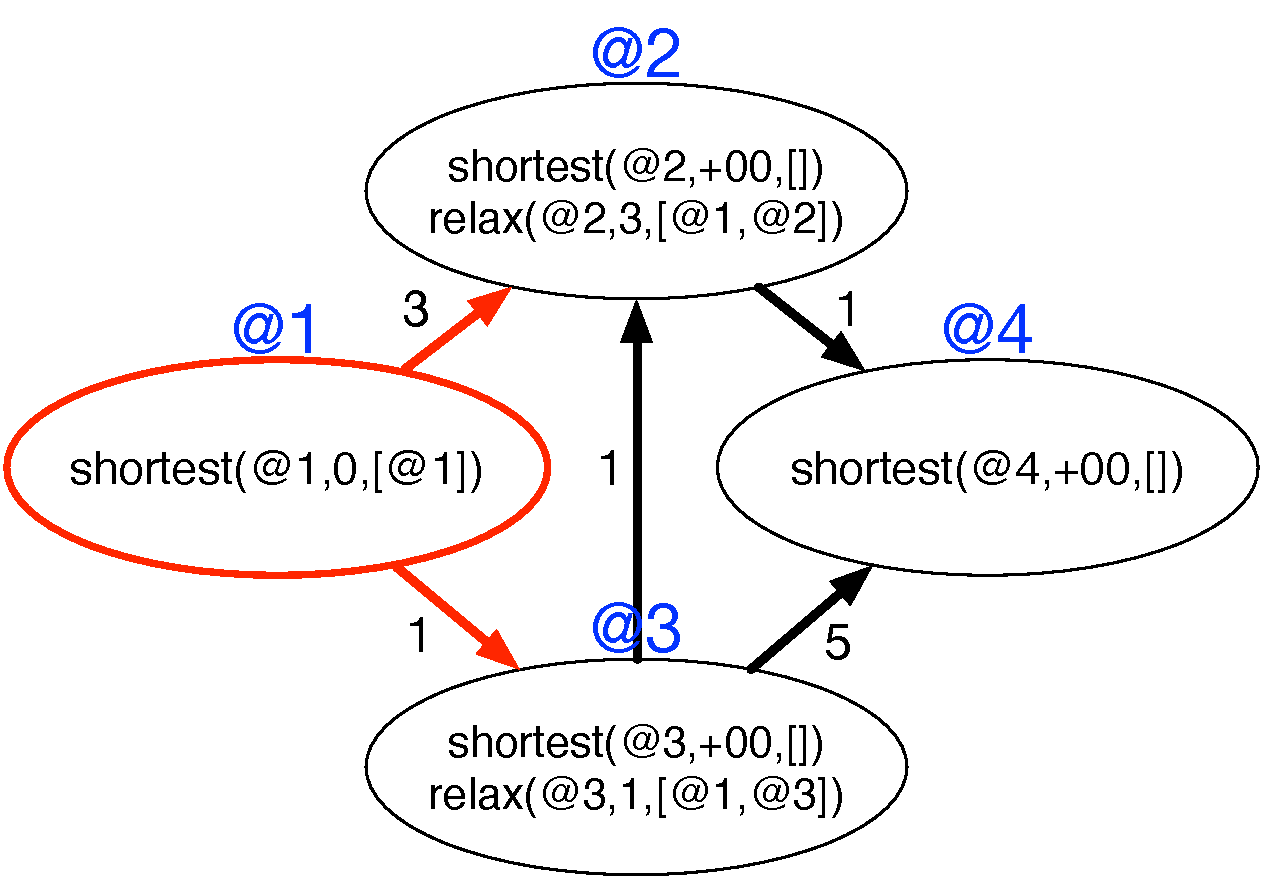
\includegraphics[width=0.3\textwidth]{figures/shortest2}}
  \subfloat[]{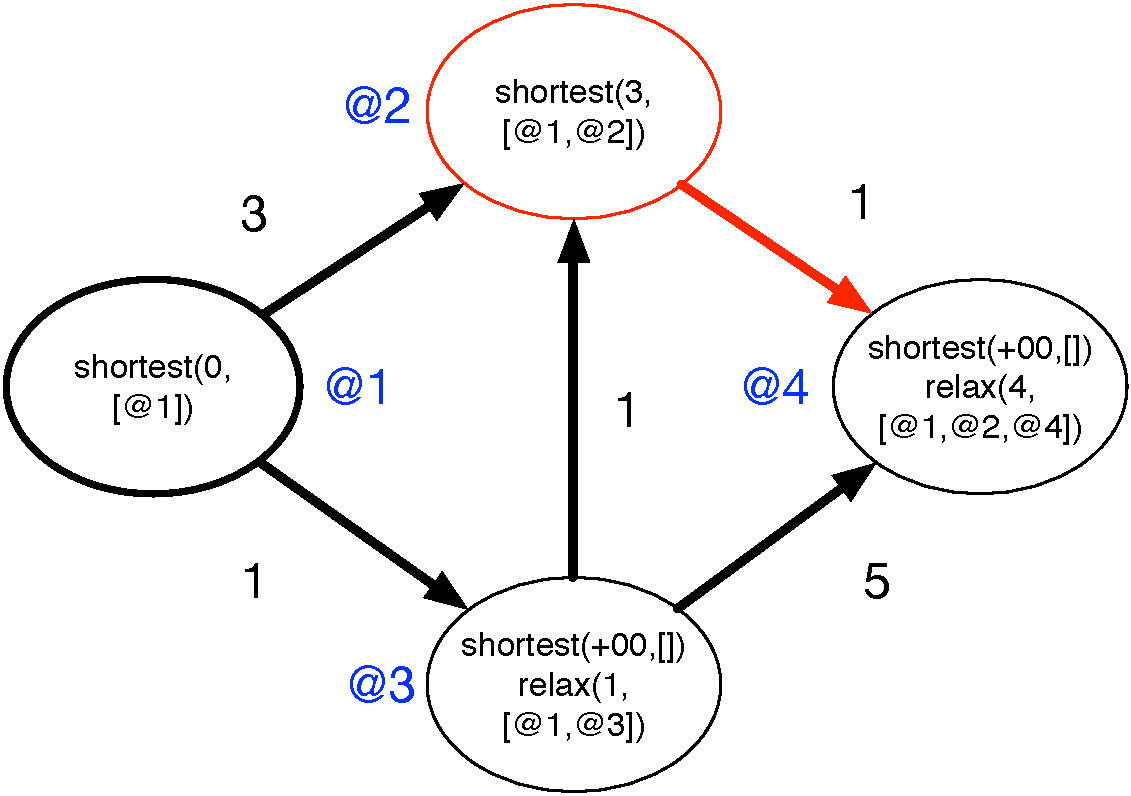
\includegraphics[width=0.3\textwidth]{figures/shortest3}}
  \subfloat[]{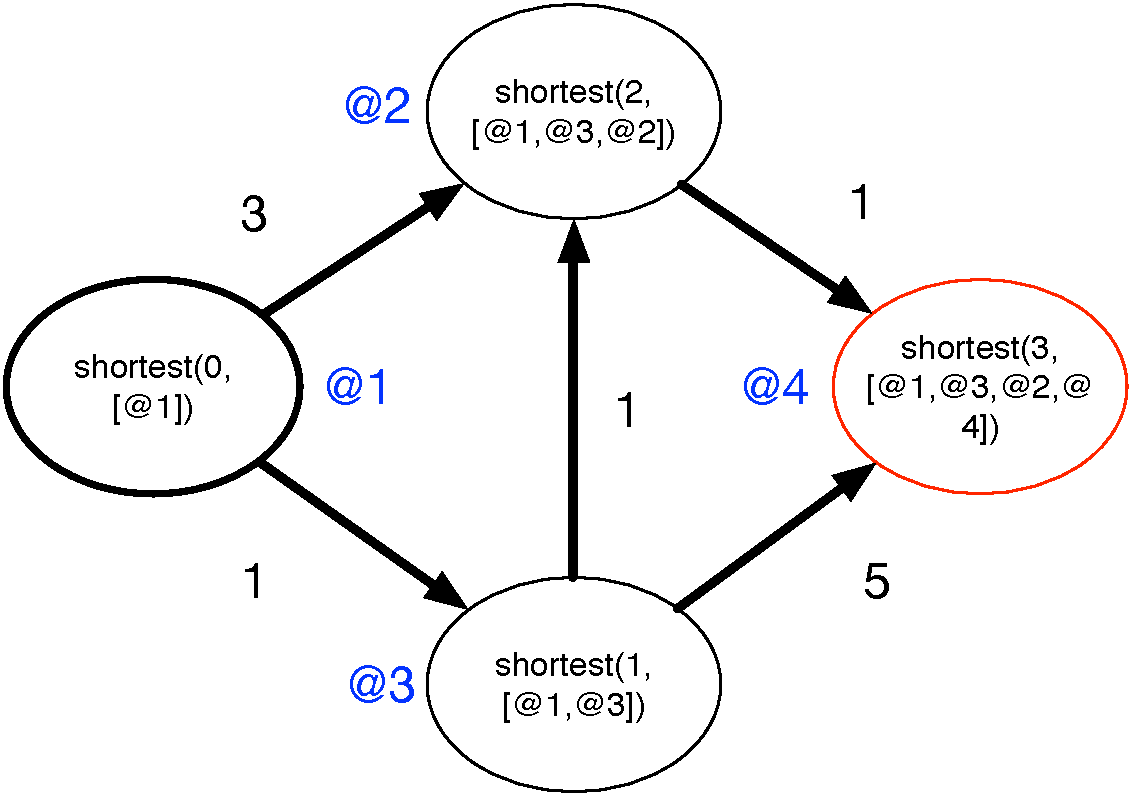
\includegraphics[width=0.3\textwidth]{figures/shortest8}}
\end{center}
\caption{Graphical representation of the SSSP program. Figure (a) represents the
   program after propagating initial distance at node \texttt{@1}, followed by
   Figure (b) where the first rule is applied in node \texttt{@3}. Figure (c)
   represents the state of the final program, where all the shortest paths
   have been computed.}
\label{fig:shortest_path_program}
\end{figure*}

The second rule of the program (lines 17-19) deals with the case where the new
distance in \texttt{relax} is not better than the current one, so it is thrown
away and the current distance is kept.

There many opportunities for concurrency in the SSSP program. For instance,
after applying rule 1 in Fig.~\ref{fig:shortest_path_program}~(a), it is
possible to either apply rules in either node \texttt{@2} or node
\texttt{@3}. In our implementation, we partition the graph into subgraphs that
are processed by multiple threads of execution. Eventually, it is no longer to
possible to apply rules and the final result present in
Fig.~\ref{fig:shortest_path_program}~(c) is achieved.

%On the other hand, LM has no natural matching of data and computation to workers (processes, threads),
%since nodes are a program abstraction and part of the program's logic.
%We view the set of nodes as a graph data structure where workers will perform work.
%A worker is able to process any node, although a node cannot be computed by more than one worker
%at the same time. This disallows the manipulation of a node by multiple workers.



\section{Coordination}
Since LM uses linear logic and supports deletion of facts, the order in which
nodes are scheduled can impact the performance and even the results of the
program.

The SSSP program present in Fig.~\ref{code:shortest_path_program} is concise and
declarative but its performance may depend in the order in which nodes are
executed. If nodes with greater distances are prioritized over other nodes, the
program will generate more \texttt{relax} facts since it will take longer to
reach the shortest distances. From Fig.~\ref{fig:shortest_path_program}, it is
clear that the best computational ordering is the following: \texttt{@1},
\texttt{@3}, \texttt{@2} and then \texttt{@4}, where only 4 \texttt{relax}
facts are generated. If we had decided to process nodes in order
\texttt{@1}, \texttt{@2}, \texttt{@4}, \texttt{@3}, \texttt{@4},
\texttt{@2}, then 6 \texttt{relax} facts would have been generated.
Therefore, the optimal solution for SSSP is to schedule the node with the
shortest distance, which is essentially the Dijkstra shortest path
algorithm~\cite{Dijkstra}. Note how it is possible to change the nature of
the algorithm by simply changing the order of node computation, but still
retain the declarative nature of the program.

We introduce the concept of \emph{coordination facts} that allow the programmer
to change how the run time schedules nodes and partitions the nodes among
threads of execution. Coordination facts can be used in the body or head of the
rules to allow the programmer to reason and change how execution is to be done.
In this fashion, we keep the language declarative because we reason logically
about the state of execution, without the need to introduce extra-logical
operators into the language that would introduce problems when attempting to prove
properties about programs.

There are two classes of coordination facts. The first class of coordination facts are
called \emph{sensing facts} and are used to sense information about the
underlying runtime system, including node placement and node scheduling.
The second kind of coordination facts are \emph{action facts} that are deleted
to apply a coordination operation in the runtime system.

\subsection{Scheduling Facts}\label{sec:fifo}

We can use action facts to change the order in which nodes are evaluated by adding
\emph{priorities}. Node priority works at the thread level
so that each thread can make a local decision about which node to execute next.
Note that, by default, nodes are picked using a FIFO approach, because that
tends to work better for most programs since older nodes tend to have more facts
to be used.

We have two kinds of priorities: a \emph{temporary priority} and a \emph{default
priority}. A temporary priority momentarily changes the default priority $D$ of a
node, so that once the node is done, the priority will default back to $D$.
Initially, all nodes have a default priority of $0$.

The following list presents the action facts available to manipulate the scheduling
decisions of the system:

\begin{itemize}
   \item \texttt{type linear set-priority(node, float)}: This sets the
   temporary priority of a node. If the node already has a priority, we only
   change the priority if the new one is higher. The programmer can
   decide if priorities are to be ordered in ascending or descending order.
   \item \texttt{type linear action add-priority(node, float)}: Increases,
   temporarily, the priority of the node.
   \item\texttt{type linear schedule-next(node)}: The work will fetch the
   highest priority node's priority $P$ from its set of nodes and set the
   action's argument node's priority as $P + 1.0$. If using the priorities in
   ascending order, we pick the lowest priority and subtract $1.0$.
   \item\texttt{type linear set-default-priority(node, float)}: Sets the default
   priority of the node.
   \item \texttt{type linear action stop-program(node)}: Immediately stops the
   execution of the whole program.
\end{itemize}

LM provides the sensing fact \texttt{priority(A, B, P)} in order to sense the
priority \texttt{P} of node \texttt{B} from node \texttt{A}.
Sensing facts are only used in the body of the rules in order
to fetch information from the runtime system.
Note that when sensing facts are deleted, they are re-derived automatically.
Logically, \texttt{set-priority} and \texttt{set-default-priority} update the
value of \texttt{priority} facts, but this done automatically by the runtime
system.

\subsubsection{Partitioning facts}

We provide several coordination facts for dealing with node partitioning among
the available threads executing the program. In terms of action
facts, we have the following:

\begin{itemize}
   \item \texttt{type linear set-cpu(node, int)}: Moves the node to a
   thread of execution.
   \item \texttt{type linear set-affinity(node, node)}: Places the first node in
   the same thread as the second node.
   \item \texttt{type linear set-moving(node)}: Allows the node to move freely
   between threads.
   \item \texttt{type linear set-static(node)}: Forces the node to stay in the
   same thread indefinitely.
\end{itemize}

For sensing facts, we have the following set of coordination facts:

\begin{itemize}
   \item \texttt{type linear cpu-id(node, node, int)}: The third argument
   indicates the thread where the node of the second argument is currently running.
   \item \texttt{type linear moving(node, node)}: Fact available if the node in the
   second argument is allowed to move between threads.
   \item \texttt{type linear static(node, node)}: Fact available if the node in
   the second argument is not allowed to move between threads.
\end{itemize}

\iffalse
\subsubsection{Global Directives}

We also provide a few global coordination statements:

\begin{description}
   \item[\texttt{priority @order ORDER.}] \texttt{ORDER} can be either \texttt{asc} or \texttt{desc}. This defines if node's are to be selected by the smallest or the greatest priority, respectively.
   \item[\texttt{priority @initial P.}] The \texttt{initial} statement informs the runtime system that all nodes must start with priority $P$. Alternatively, the programmer can define an \texttt{set-priority(A, P)} axiom.
   \item[\texttt{priority @static.}] The \texttt{static} priority tells the runtime system that the partition of nodes among workers is to be used until the end of program. 
\end{description}

\fi


\section{Experimental Results and Discussion}
\subsection{Absolute runtime}

In the paper~\cite{cruz-ppdp14}, the LM virtual machine was measured and
compared against implementations of similar programs but written in other
languages. For instance, the LBP program was found to be around 2 times slower
than GraphLab, while N Queens program was found to be around 10 to 15 slower
than a sequential C implementation. Some of those programs were compared against
a Python implementations and LM faired fairly well. In this section, we measure
the impact of the coordination mechanisms we have implemented for the new
virtual machine.

Fig.~\ref{results:comparison1}

\begin{figure}[h!]
   \begin{center}
      \subfloat[]{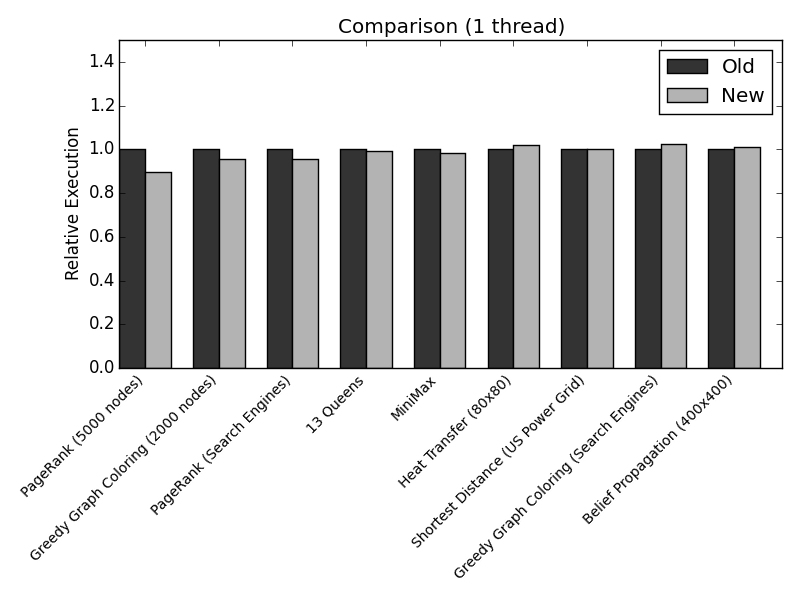
\includegraphics[width=9cm]{results/comparison1.png}}
   \end{center}
   \caption{Measuring the overhead of coordination mechanisms. The \textbf{Old}
   bars represent the performance of the original virtual machine, while
   \textbf{New} is the relative performance of the new version that includes
   coordination mechanisms. Most programs show little to no degradation in
   performance.}
   \label{results:comparison1}
\end{figure}


\section{Related Work}
Recently, there has been an increasing interest in declarative and data-centric
languages. MapReduce~\cite{Dean:2008:MSD:1327452.1327492}, for instance, is a
popular data-centric programming model that is optimized for large clusters. The
scheduling and data sharing model is very simple: in the \emph{map phase}, data
is transformed at each node and the result reduced to a final result in the
\emph{reduce phase}. Like LM, many programming systems model the program as a
graph where computation will be performed. The Dryad
system~\cite{Isard:2007:DDD:1272996.1273005} combines computational vertices
with communication channels (edges) to form a data-flow graph. The program is
scheduled to run on multiple computers or cores and data is partitioned
automatically during runtime.

Many programming languages follow the so-called \emph{coordination
paradigm}~\cite{Papadopoulos98coordinationmodels}, a form of distributed
programming that divides execution in two parts: \emph{computation}, where the actual
computation is performed, and \emph{coordination}, which deals with
communication and cooperation between processing units. This paradigm attempts
to clearly distinguish between these two parts by providing abstractions for
coordination in an attempt to provide architecture and system-independent forms
of communication.  

Linda~\cite{linda} is probably the most famous coordination model. Linda
implements a data-driven coordination model and features a \emph{tuple space}
that can be manipulated using the following coordination directives:
\texttt{out(t)} writes a tuple \texttt{t} into the tuple space; \texttt{in(t)}
reads a tuple using the template \texttt{t}; \texttt{rd(t)} retrieves a copy of
the tuple \texttt{t} from the tuple space; and \texttt{eval(p)} puts a process
\texttt{p} in the tuple space and executes it in parallel. 
Linda is be implemented on top of many
popular languages by simply creating a communication and storage mechanism for
the tuple space and then adding the directives as a language library.

Another coordination language is Delirium~\cite{Delirium}, where instead of being
embbeded in another language like Linda, it actually embeds operators other
languages inside Delirium. The advantages of Delirium are improved abstraction
and easier debugging because sequential operators are isolated from the
coordination language.

Linda and Delirium are limited in the sense that the programmer can only
coordinate the scheduling of processing units, while the placement of data is
left to the implementation. LM also differs from those languages since it
raises the abstraction level from the processing units to nodes of a graph,
which are part of the program logic.
Furthermore, the language LM is both the coordination and the computation
language and there is no distinction between them.

\iffalse
GraphLab~\cite{GraphLab2010} is a C++ framework for developing parallel machine
learning algorithms. GraphLab allows nodes to
have read/write access to different scopes through different concurrent access
models in order to balance performance and data consistency. While some programs
only need to access the local node's data, others may need to update edge
information. Each consistency model will provide different guarantees that are
better adapted to some algorithms. GraphLab provides different schedulers
that dictate the order in which node's are computed, which is a rudimentary form
of coordination. Later in this paper, we will show how certain GraphLab's
schedulers can be easily implemented in LM through the use of coordination
facts.
\fi


\section{Conclusions}

\section{Acknowledgements}

\input{ack}

\bibliographystyle{abbrvnat}
\bibliography{refs}

\end{document}
